\documentclass[UTF8,11pt,a4paper]{ctexart}
\usepackage[margin=2.5cm]{geometry}
\usepackage{amsmath,amssymb,booktabs,graphicx,hyperref}
\setCJKmainfont{Songti SC}
\setlength{\parindent}{2em}
\newcommand{\RunID}{q1-20260910T142542Z}
\newcommand{\QOneCost}{35,126.9486}
\newcommand{\NoStorageCost}{48,052.0466}
\newcommand{\RuleCost}{46,428.9954}
\newcommand{\QOneGrid}{59,482.6990}
\newcommand{\Saving}{26.8981}
\newcommand{\TotalLoad}{111,024.8081}
\newcommand{\TotalPV}{55,482.8357}
\newcommand{\ChargeTotal}{20,740.6661}
\newcommand{\DischargeTotal}{16,799.9396}
\newcommand{\EfficiencyCost}{33,801.4955}
\newcommand{\PointCost}{35,042.5400}

\title{微网购电调度：题面审计与第一问实算报告}
\author{}
\date{2026年9月10日}
\begin{document}
\pagestyle{plain}
\maketitle
\noindent\textbf{状态：}第一轮模型与结果审阅稿。模板时间标签存在未澄清歧义；此文不是最终竞赛论文。运行编号：\texttt{\RunID}。

\section{四问任务与已核验输入}
第一问使用附件1已给的日电价、负载与光伏预测，0点规划全天购电，要求不缺电且首末储电量相同。第二问仅凭截至0点的历史预测负载和光伏，普通购电按计划收费，缺口按五倍电价紧急购买。第三问加入每天0、6、12、18点发布的光伏预报，以及增减合同费用；必须分离额外信息与修改合同的价值。第四问在波动电价下重做第二、三问，题面未明确未来价格提前可见。

全部3页题面、4个数据附件和5个模板均已读取。实际数据覆盖365日、每天144个10分钟区间；预报有1460次发布、每次24个整点，共35040值。第二至四问正式评估为2月1日至12月31日334日，不是仅计算四个展示日。数值无缺失、无负值，电价均为正。原件已按用途迁移，11份原件哈希不变。

\section{时间与计量假设}
原数据标签00:10至24:00暂解释为此前10分钟的平均功率/交付价格；内部使用左闭右开144区间与145个储能端点，不套用夏令时。功率乘$1/6$小时换为kWh。模板却把购电标签从00:10--00:20排到次日00:00--00:10，整体错位10分钟。导出保留原标签并单独提供逐格映射，不能声称已消除官方语义歧义。

暂按充、放单程效率均为0.9；充放电量及5000kW功率均为交流母线侧，储电量为电池内部电量。往返90\%的解释另外计算敏感性。富余能量可以不用，合同仍收费，无售电收入。第一问初末储电量按总指令取6000kWh。

\section{第一问模型}
对$t=0,\ldots,143$，定义购电$q_t$、充电$c_t$、放电$d_t$、未利用能量$w_t$，均为区间kWh；内部储电量$E_t$为kWh，$z_t\in\{0,1\}$。负载与光伏区间电量分别为$\ell_t,v_t$，电价$p_t$为元/kWh。模型为
\begin{align}
\min\quad &\sum_{t=0}^{143}p_tq_t,\\
q_t+v_t+d_t&=\ell_t+c_t+w_t,\\
E_{t+1}&=E_t+0.9c_t-d_t/0.9,\\
1200\le E_t&\le10800,\quad E_0=E_{144}=6000,\\
0\le c_t&\le(5000/6)z_t,\\
0\le d_t&\le(5000/6)(1-z_t),\quad q_t,w_t\ge0.
\end{align}
采用SciPy/HiGHS求解MILP，另以相同数据、初末状态和约束解LP松弛作为下界。简单规则基线在0--6点充电、16点以后放电并恢复初始储量；它与优化策略使用相同物理条件。

\section{真实结果与验证}
全天负载\TotalLoad\ kWh，光伏\TotalPV\ kWh。MILP计划购电\QOneGrid\ kWh，费用\QOneCost\ 元；充电\ChargeTotal\ kWh，放电\DischargeTotal\ kWh，无未利用能量。无储能成本\NoStorageCost\ 元，规则基线\RuleCost\ 元，MILP较无储能节省\Saving\%。

HiGHS返回optimal、MIP gap为0；MILP目标与同约束LP下界一致。独立复算母线残差约$1.14\times10^{-13}$kWh，SOC递推残差约$8.60\times10^{-13}$kWh；无越界、无同时充放电，首末6000kWh，费用独立对账通过。这证明当前离散假设模型的数值可行性与最优性，不是微网现场验证。

\begin{center}
表1：指定时段及全天购电结果（区间电量单位：kWh）\\[4pt]
\small\begin{tabular}{lrlrlr}\toprule 时间段 & 购电量 & 时间段 & 购电量 & 时间段 & 购电量\\\midrule
10:00--10:10 & 0.0000 & 12:00--12:10 & 480.4124 & 14:00--14:10 & 0.0000\\
16:00--16:10 & 445.4316 & 18:00--18:10 & 531.8940 & 20:00--20:10 & 0.0000\\
\midrule\multicolumn{2}{c}{全天购电量/kWh} & 59,482.6990 & \multicolumn{2}{c}{全天购电费/元} & 35,126.9486\\
\bottomrule\end{tabular}

\par\medskip
表2：充放电和首末储电量（单位：kWh）\\[4pt]
\small\begin{tabular}{lrrlrr}\toprule 时间段 & 充电量 & 放电量 & 时间段 & 充电量 & 放电量\\\midrule
0:00--4:00 & 4500.0000 & 0.0000 & 4:00--8:00 & 833.3333 & 6365.8412\\
8:00--12:00 & 4787.9643 & 1702.9970 & 12:00--16:00 & 5286.0352 & 91.1014\\
16:00--20:00 & 0.0000 & 5780.1319 & 20:00--24:00 & 5333.3333 & 2859.8681\\
\midrule\multicolumn{2}{c}{0:00储电量} & 6000 & \multicolumn{2}{c}{24:00储电量} & 6000\\
\bottomrule\end{tabular}

\end{center}
\noindent 表中使用内部真实时间区间，充/放为交流母线侧。0点及24点内部储电量均为6000kWh。

\begin{figure}[htbp]\centering
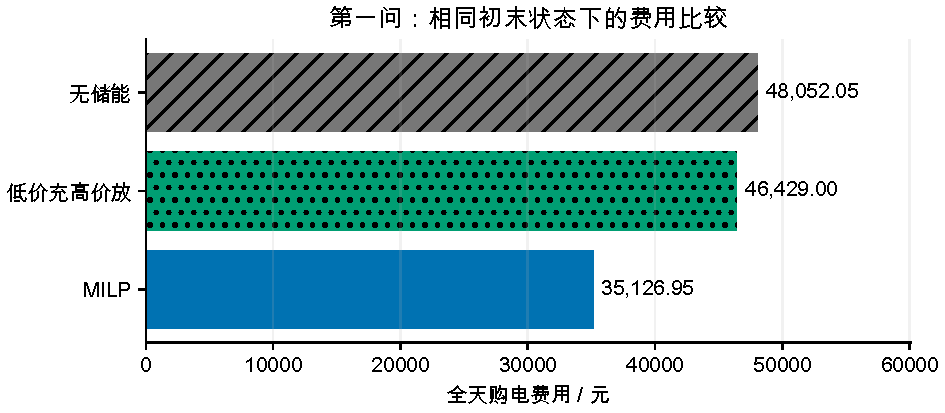
\includegraphics[width=0.92\linewidth]{../../figures/q1/q1_cost.pdf}
\caption{相同物理参数与首末状态下的费用。数据直接读取运行结果，柱形零基线。}
\end{figure}

\begin{figure}[htbp]\centering
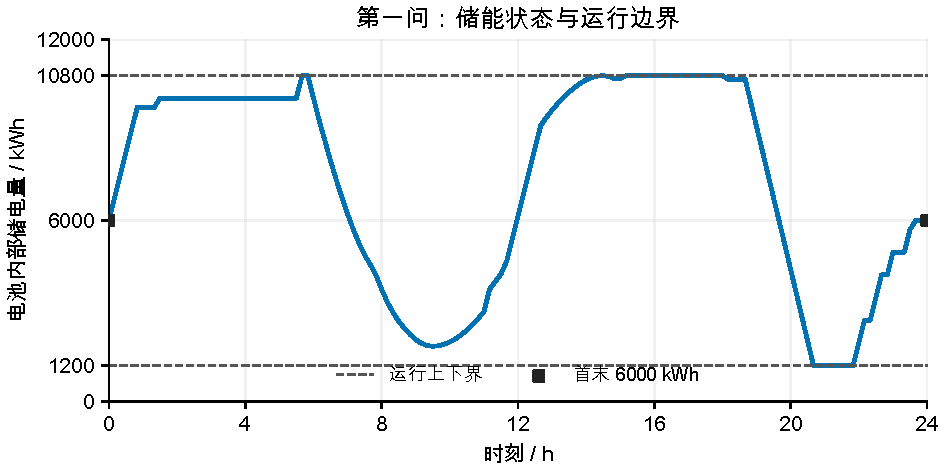
\includegraphics[width=0.95\linewidth]{../../figures/q1/q1_soc.pdf}
\caption{145个状态端点。午间低价段不必立即充满，后续光伏富余需要容量；全日最低价段是否充满必须按实际轨迹判断。}
\end{figure}

\section{敏感性与下一阶段}
将90\%解释为往返效率，单程取$\sqrt{0.9}$，成本为\EfficiencyCost\ 元。将功率解释为周期瞬时端点、用非负线性积分重构，成本为\PointCost\ 元。两者均重新求解并核验，不替换主结果。

后续使用按日滚动历史验证选预测模型和安全裕量；规划器只收到当时可见信息，当前区间控制器与未来真值隔离。第三问分别实现原费用保留加违约费A和取消退款后罚费B，累计合同事件而不重复收原费。第四问主采用因果预测价格，提前知道当日价格只作为不同信息条件实验。后续已执行进度与结果以\texttt{context/BACKTEST\_REPORT.md}和真实输出为准，未完成部分不在本报告预填结果。

\section*{AI工具使用声明}
本轮使用Codex辅助阅读题面、审计附件、检索本地历史方法、提出模型和假设、编写优化及验证程序、执行实验、生成图表和本报告。核心模型与结果仍需参赛队员逐项人工核验；自动测试不等于人工审核。具体部署模型版本未独立核验，不编造版本号。详见独立的AI工具使用详情文件。本文没有宣称已经完成队员人工审核。
\end{document}
